\begin{figure*}[t]
\centering
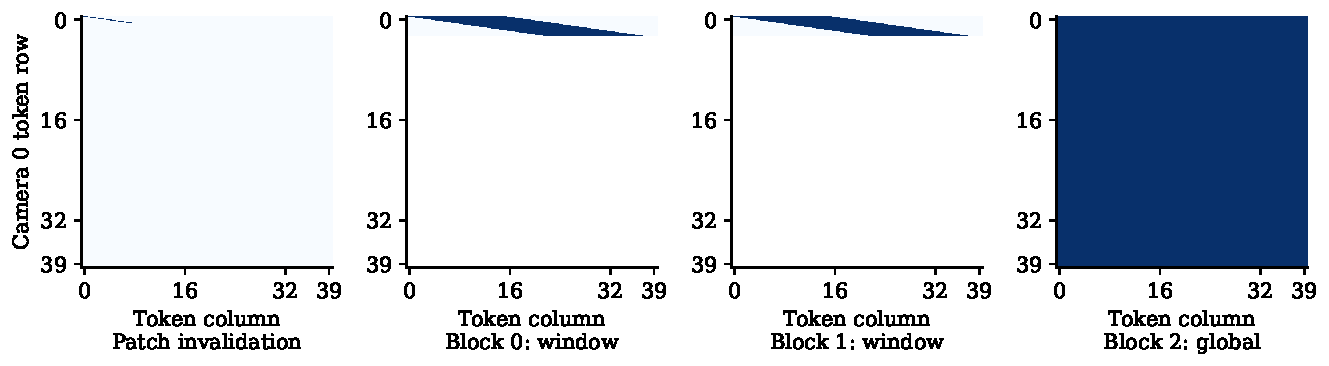
\includegraphics[width=\textwidth]{m2_a.pdf}
\caption{Actual dependency closure for one changed input patch in camera 0: dark blue marks token recomputation before window blocks 0/1 and global block 2. Horizontal and vertical coordinates are token column and row.}
\label{fig:m2-a}
\end{figure*}

\begin{figure*}[t]
\centering
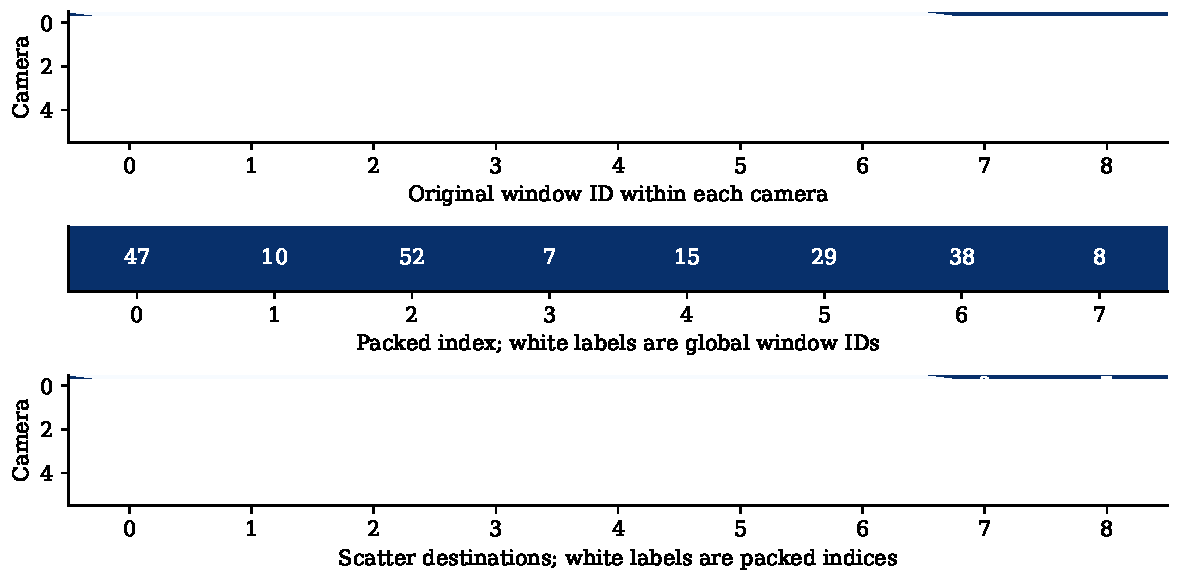
\includegraphics[width=\textwidth]{m2_b.pdf}
\caption{Actual measured update IDs (8 of 54) in camera-major layout. The packed batch shows global source IDs; destination cells show packed indices to verify scatter order. Each camera has nine windows.}
\label{fig:m2-b}
\end{figure*}

\begin{figure}[t]
\centering
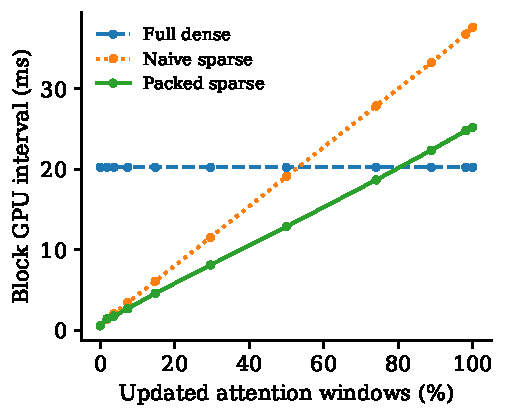
\includegraphics[width=\linewidth]{m2_c.pdf}
\caption{Controlled deployed-weight EVA block 0 on RTX 3090. Medians of 20 executions per shape, after five warmups for Full/Packed and three for Naive; one seeded changed-window mask per sparse count. The shape-invariant dense reference is measured once (20 executions) and repeated across x. Intervals include packing, cache copy, scatter and launch gaps.}
\label{fig:m2-c}
\end{figure}

\begin{figure}[t]
\centering
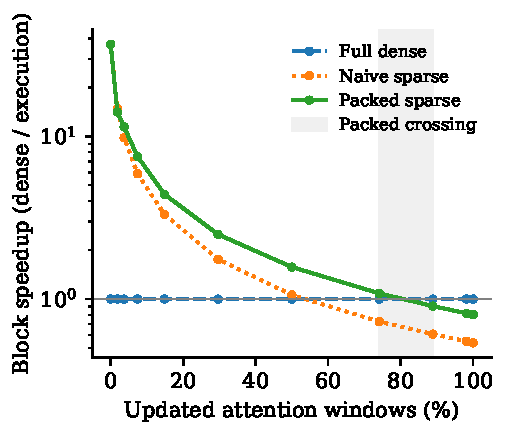
\includegraphics[width=\linewidth]{m2_d.pdf}
\caption{Block speedup from the same median costs/protocol as (c); the same dense reference is reused. Shading brackets the measured packed-sparse median crossing at 74.1 to 88.9 percent updated windows; it does not assert a threshold at an unmeasured count.}
\label{fig:m2-d}
\end{figure}

\begin{figure}[t]
\centering
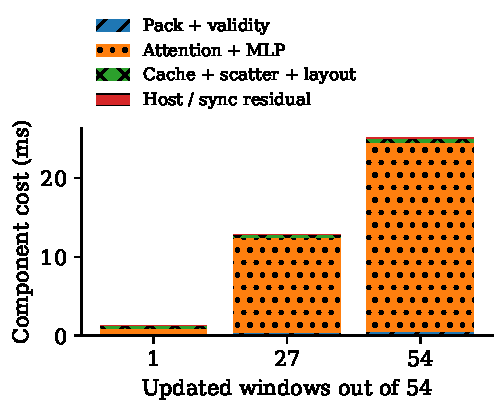
\includegraphics[width=\linewidth]{m2_e.pdf}
\caption{EVA block 0 on RTX 3090: component-wise medians over 20 instrumented executions for each count. The stack sums marginal component medians and need not equal the median complete wall time. Host/synchronization residual is wall minus event intervals, not an independent device kernel. Hatching distinguishes components in grayscale.}
\label{fig:m2-e}
\end{figure}

\begin{figure*}[t]
\centering
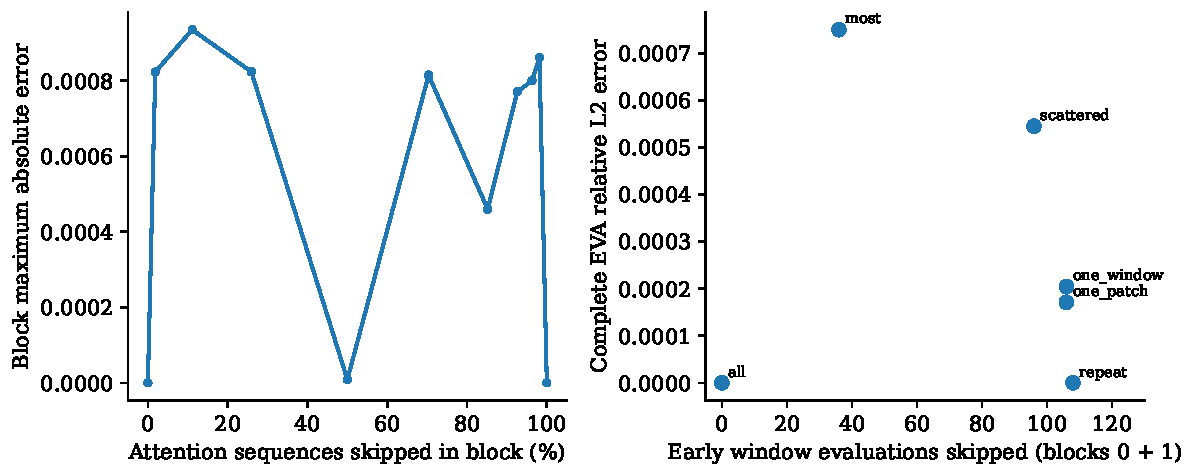
\includegraphics[width=\textwidth]{m2_f.pdf}
\caption{Controlled errors versus dependency-certified unchanged window evaluations skipped, not deliberately omitted changed work. Each sparse count uses one seeded changed-window mask. All six complete-EVA cases pass the layerwise independent dense precision envelope. The right panel counts actual block-0/1 skipped window evaluations; later blocks remain dense.}
\label{fig:m2-f}
\end{figure*}

\begin{figure*}[t]
\centering
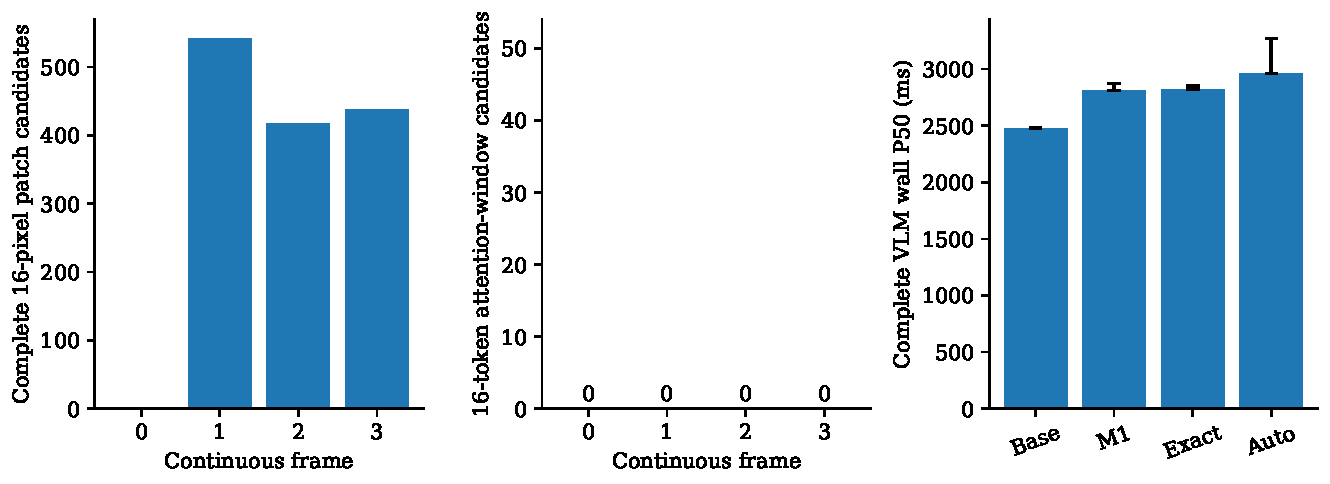
\includegraphics[width=\textwidth]{m2_g.pdf}
\caption{Real M1, four unique continuous nuScenes frames from one scene. Attention-window candidate counts are [0, 0, 0, 0]; accepted/skipped windows are also zero, so Exact/Auto use dense fallback and output equality validates that fallback. Base is original OmniDrive, M1 adds observation only, Exact adds strict M2, Auto adds cost-based M2. Bars are complete VLM wall P50; upper caps mark P95 over eight frame timings per arm: two four-frame replays after one warmup replay, including each replay reset frame. All M1/M2 costs are included. This evidence is separate from controlled sparse results.}
\label{fig:m2-g}
\end{figure*}